This section illustrates how the various subsystems interact within the SCARA robot arm. Each flow of data is
identified with an arrow to the direction of the subsystem it sends data towards, as well as indicates what sort of data is being transfered. The subsections provide a high level
overview of the system and the data flows between each of the layers and subsystems as well as
describe how individual data elements are used. 

\begin{figure}[h!]
	\centering
 	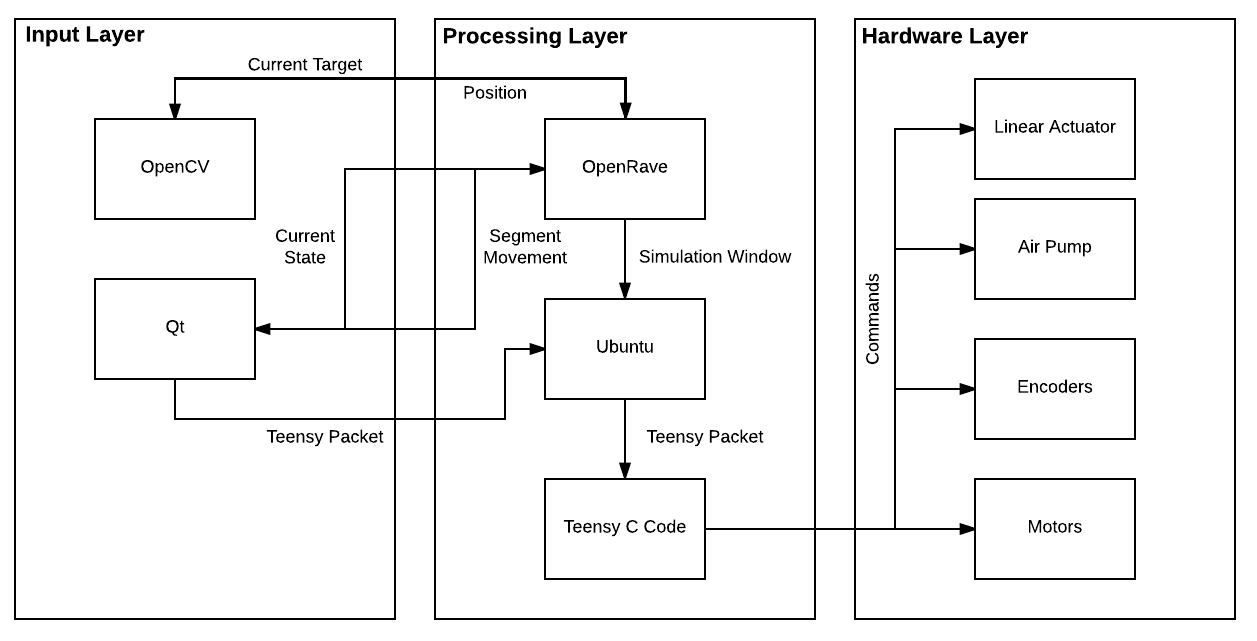
\includegraphics[width=\textwidth]{images/ADS_dataflow}
 \caption{A data flow diagram of the arm}
\end{figure}

\subsection{Data Flow Diagram}
The data flow diagram consists of three layers. Data starts at the Input Layer which is inputted through but the GUI application and the camera with OpenCV. The input layer then sends to the Processing
Layer which is responsible handling and calculating the input data. Then, the processing layer will send its commands to the Hardware layer, which will then execute these commands physically as output.